\chapter{Introduction}
%\label{\detokenize{overview/introduction/main:introduction}}\label{\detokenize{overview/introduction/main::doc}}
This book aims to introduce readers to programming for mathematics.

It is assumed that readers are used to solving high school mathematics problems
of the form:


Given the function \(f:\mathbb{R}\to\mathbb{R}\) defined by
\(f(x) = x ^ 2 - 3 x + 1\) obtain the global minima of the function.


To solve this we need to apply our \textbf{mathematical knowledge} which tells us to:

\begin{enumerate}
\item Differentiate \(f(x)\) to get \(\frac{df}{dx}\);
\item Equate \(\frac{df}{dx}=0\);
\item Use the second derivative test on the solution to the previous equation.
\end{enumerate}

For each of those 3 steps we will usually make use of our \textbf{mathematical
techniques}:
\begin{enumerate}
\item Differentiate \(f(x)\):

\begin{equation*}
\begin{split}\frac{df}{dx} = 2 x - 3\end{split}
\end{equation*}
\item Equate \(\frac{df}{dx}=0\):
\begin{equation*}
\begin{split}2x-3 =0 \Rightarrow x = 3/2\end{split}
\end{equation*}
\item Use the second derivative test on the solution:
\begin{equation*}
\begin{split}\frac{d^2f}{dx^2} = 2 > 0\text{ for all values of }x\end{split}
\end{equation*}
Thus \(x=3/2\) is the global minima of the function.

\end{enumerate}

As we progress as mathematicians \textbf{mathematical knowledge} is more prominent
than \textbf{mathematical technique}: often knowing what to do is the real problem as
opposed to having the technical ability to do it.

This is what this book will cover: \textbf{programming} allows us to instruct a
computer to carry out mathematical techniques.

We will for example learn how to solve the above problem by instructing a
computer which \textbf{mathematical technique} to carry out.

\textbf{This book covers how to give the correct instructions to a
computer.}

The following is an example, do not worry too much about the specific code used
for now:


\textbf{Differentiate \(f(x)\) to get \(\frac{df}{dx}\)}

\begin{pyin}
import sympy as sym

x = sym.Symbol("x")
sym.diff(x ** 2 - 3 * x + 1, x)
\end{pyin}

\[
    2x - 3
\]

\textbf{Equate \(\frac{df}{dx}=0\)}

\begin{pyin}
sym.solveset(2 * x - 3, x)
\end{pyin}

\[
\left\{\frac{3}{2}\right\}
\]

\section{Use the second derivative test on the solution}
%\label{\detokenize{overview/introduction/main:use-the-second-derivative-test-on-the-solution}}

\begin{pyin}
sym.diff(x ** 2 - 3 * x + 1, x, 2)
\end{pyin}

\[2\]

Figure~\ref{fig:knowledge_vs_technique} shows a summary.

\begin{figure}[htbp!]
\centering

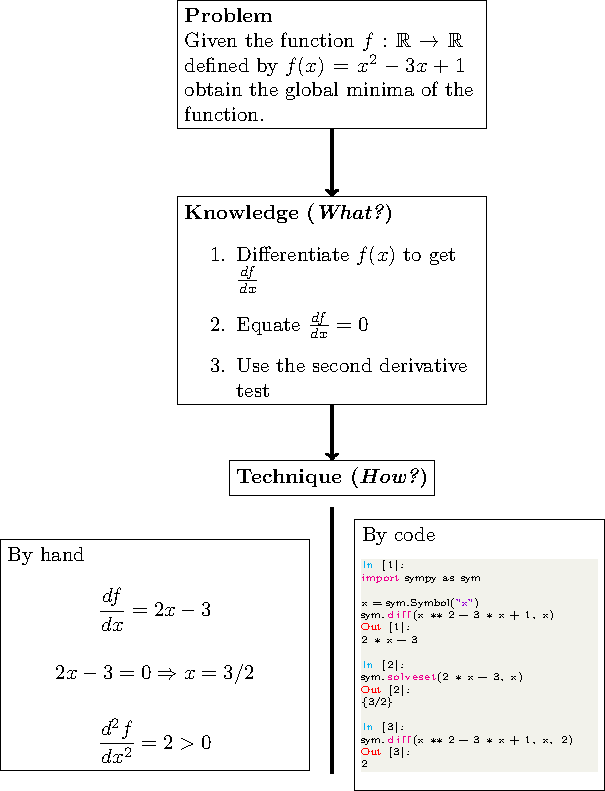
\includegraphics[width=0.75\textwidth]{assets/knowledge_vs_technique/main.pdf}
\caption{Knowledge versus technique in this
    book.}\label{fig:knowledge_versus_technique}
\end{figure}

\section{How this book is structured}
%\label{\detokenize{overview/structure/main:how-this-book-is-structured}}\label{\detokenize{overview/structure/main::doc}}

Most programming texts introduce readers to the building blocks of
programming and build up to using more sophisticated tools for a specific
purpose.

This is akin to teaching someone how to forge metal so as to make a nail and
then slowly work our way to using more sophisticated tools such as power tools
to build a house.

This book will do thing in a different way: we will start with using and
understanding tools that are helpful to mathematicians. In the later part of the
book we will cover the building blocks and you will be able to build your own
sophisticated tools.

The book is in three parts:
\begin{enumerate}
\item Tools for mathematics;
\item Building tools;
\item Further information.

\end{enumerate}

The first part of the book will not make use of any novel mathematics.
Instead we will consider a number of mathematics problem that are often covered
in secondary school.

\begin{itemize}
    \item Algebraic manipulation
    \item Calculus (differentiation and integration)
    \item Combinatorics (permutations and combinations)
    \item Probability
    \item Linear algebra
    \item Sequences
    \item Statistics
    \item Differential equations
\end{itemize}

The questions we will tackle will be familiar in their presentation and
description. \textbf{What will be different} is that no \textbf{by hand} calculations will
be done. We will instead carry them all out using a programming language.

In the second part of the book you will be encouraged to build your own tools
to be able to tackle a problem type of your choice.

Every chapter will have 4 parts:

\begin{itemize}
\item A tutorial: you will be walked through solving a problem. You will be
specifically told what to do and what to expect.

\item A how to section: this will be a shorter more succinct section that will
detail how to carry out specific things.

\item 
A further information section: this will be a section with references to
further resources as well as background information about specific things in
the chapter and answers to common questions.

\item
An exercise section: this will be a number of exercises that you can work on.

\end{itemize}


\section{How to use this book}
%\label{\detokenize{overview/how_to_use_this_book/main:how-to-use-this-book}}\label{\detokenize{overview/how_to_use_this_book/main::doc}}
Readers are welcome to use this book in any way they find useful however it is
designed with the following suggestion in mind:
\begin{itemize}
\item Start by following along with the tutorial. Carrying out the steps and
observing the outcomes. It is not expected that a reader gains a deep
understanding of a given topic when working through the tutorial. The goal
here is to achieve some level of familiarity.

\item After the tutorial, work through the how to section. It is through this
section that a deeper understanding is to be gained by making connections to
steps taking in the tutorial. \textbf{After working through the how to section it is
hoped that the reader would understand all steps taken in the tutorial}.

\item The exercise section is an opportunity for the reader to practice the topics
in the how to section. Solutions are available in this section as well.

\item After working through those three section it is possible that some readers
have further questions or would like to find more information about a
given topic. This is covered in the further information section.

\end{itemize}

